\documentclass{article}\usepackage[]{graphicx}\usepackage[]{color}
%% maxwidth is the original width if it is less than linewidth
%% otherwise use linewidth (to make sure the graphics do not exceed the margin)
\makeatletter
\def\maxwidth{ %
  \ifdim\Gin@nat@width>\linewidth
    \linewidth
  \else
    \Gin@nat@width
  \fi
}
\makeatother

\definecolor{fgcolor}{rgb}{0.345, 0.345, 0.345}
\newcommand{\hlnum}[1]{\textcolor[rgb]{0.686,0.059,0.569}{#1}}%
\newcommand{\hlstr}[1]{\textcolor[rgb]{0.192,0.494,0.8}{#1}}%
\newcommand{\hlcom}[1]{\textcolor[rgb]{0.678,0.584,0.686}{\textit{#1}}}%
\newcommand{\hlopt}[1]{\textcolor[rgb]{0,0,0}{#1}}%
\newcommand{\hlstd}[1]{\textcolor[rgb]{0.345,0.345,0.345}{#1}}%
\newcommand{\hlkwa}[1]{\textcolor[rgb]{0.161,0.373,0.58}{\textbf{#1}}}%
\newcommand{\hlkwb}[1]{\textcolor[rgb]{0.69,0.353,0.396}{#1}}%
\newcommand{\hlkwc}[1]{\textcolor[rgb]{0.333,0.667,0.333}{#1}}%
\newcommand{\hlkwd}[1]{\textcolor[rgb]{0.737,0.353,0.396}{\textbf{#1}}}%
\let\hlipl\hlkwb

\usepackage{framed}
\makeatletter
\newenvironment{kframe}{%
 \def\at@end@of@kframe{}%
 \ifinner\ifhmode%
  \def\at@end@of@kframe{\end{minipage}}%
  \begin{minipage}{\columnwidth}%
 \fi\fi%
 \def\FrameCommand##1{\hskip\@totalleftmargin \hskip-\fboxsep
 \colorbox{shadecolor}{##1}\hskip-\fboxsep
     % There is no \\@totalrightmargin, so:
     \hskip-\linewidth \hskip-\@totalleftmargin \hskip\columnwidth}%
 \MakeFramed {\advance\hsize-\width
   \@totalleftmargin\z@ \linewidth\hsize
   \@setminipage}}%
 {\par\unskip\endMakeFramed%
 \at@end@of@kframe}
\makeatother

\definecolor{shadecolor}{rgb}{.97, .97, .97}
\definecolor{messagecolor}{rgb}{0, 0, 0}
\definecolor{warningcolor}{rgb}{1, 0, 1}
\definecolor{errorcolor}{rgb}{1, 0, 0}
\newenvironment{knitrout}{}{} % an empty environment to be redefined in TeX

\usepackage{alltt}

\usepackage{fancyhdr} % Required for custom headers
\usepackage{lastpage} % Required to determine the last page for the footer
\usepackage{extramarks} % Required for headers and footers
\usepackage{graphicx} % Required to insert images
\usepackage{hyperref}
\usepackage{amsmath} %for binomial pdf
\usepackage{parskip} % so that there's space bw paragraphs
\usepackage{float}
\usepackage{amsfonts}

% Margins
\topmargin=-0.45in
\evensidemargin=0in
\oddsidemargin=0in
\textwidth=6.5in
\textheight=9.0in
\headsep=0.25in 

\linespread{1.1} % Line spacing

% Set up the header and footer
\pagestyle{fancy}
\lhead{STAT 534: Spatial} % Top left header
\chead{HW 5} % Top center header
\rhead{Andrea Mack} % Top right header
\lfoot{02/17/2017} % Bottom left footer
\cfoot{} % Bottom center footer
\rfoot{Page\ \thepage\ of\ \pageref{LastPage}} % Bottom right footer
\renewcommand\headrulewidth{0.4pt} % Size of the header rule
\renewcommand\footrulewidth{0.4pt} % Size of the footer rule

\setlength\parindent{0pt} % Removes all indentation from paragraphs
\setlength\parskip{0.5cm}
\restylefloat{table}

%----------------------------------------------------------------------------------------
%	DOCUMENT STRUCTURE COMMANDS
%	Skip this unless you know what you're doing
%----------------------------------------------------------------------------------------

% Header and footer for when a page split occurs within a problem environment
\newcommand{\enterProblemHeader}[1]{
\nobreak\extramarks{#1}{#1 continued on next page\ldots}\nobreak
\nobreak\extramarks{#1 (continued)}{#1 continued on next page\ldots}\nobreak
}

% Header and footer for when a page split occurs between problem environments
\newcommand{\exitProblemHeader}[1]{
\nobreak\extramarks{#1 (continued)}{#1 continued on next page\ldots}\nobreak
\nobreak\extramarks{#1}{}\nobreak
}


%----------------------------------------------------------------------------------------%
\IfFileExists{upquote.sty}{\usepackage{upquote}}{}
\begin{document}



\begin{enumerate}
\item %1
{\it Let $\gamma$(si,sj)= $\gamma$(hij) be a semivariogram for a second-order stationary spatial process.}
\begin{enumerate} 
\item %1a
{\it Show that}


\vspace{3in}

\item %1b
{\it Show that}

\vspace{3in}
\end{enumerate}

\item %2
{\it Matheron’s semivariogram estimator is}

\vspace{1in}

{\it where N(h)= {(si,sj):h=si-sj} and |N(h)| is the number of pairs in the set N(h).}

\begin{enumerate}
\item %2a
{\it Let Z(s) = $\mu$ + e(s) where E [e(s)] = 0 with  Z (h) =  e(h) (adding a constant to the random error terms does not change the variance/covariance properties of the process). Show that $\hat{\gamma}$(h) is unbiased for $\gamma_{z}$(h). That is, show E [ $\hat{\gamma}$(h)] =  $\gamma_{z}$(h). Hint: Show that under an assumption of a constant mean}

\vspace{4in}

\item {\it We pointed out in class that Matheron’s Estimator is biased in the presence of trend. Let Z(s) = $\mu$(s) + e(s) with E [e(s)] = 0 and  $\gamma_{z}$(h) =  $\gamma_{e}$(h). Show}

\vspace{4in}

\item %2c
{\it Consider the (very) simple model Zi = 10 + ei where the ei’s are independent normally distributed error terms with variance  $\sigma^{2}$ = 81. We have a pure nugget effect model  $\gamma_{z}$(h) =  $\gamma_{e}$(h) = 81. Simulate 100 observations of Zi and calculate the empirical semi- variogram assuming the observations are on a one-dimensional transect.}

{\it Compare what you see in the plot to the true  $\gamma_{z}$(h). Is the result consistent with part (a) above? Why or why not?}

\begin{knitrout}\footnotesize
\definecolor{shadecolor}{rgb}{0.969, 0.969, 0.969}\color{fgcolor}\begin{kframe}
\begin{alltt}
\hlkwd{set.seed}\hlstd{(}\hlnum{123}\hlstd{)}
\hlkwd{library}\hlstd{(geoR)}
    \hlstd{Zdat}\hlkwb{<-}\hlnum{10}\hlopt{+}\hlkwd{rnorm}\hlstd{(}\hlnum{100}\hlstd{,}\hlnum{0}\hlstd{,}\hlnum{9}\hlstd{)}
    \hlstd{i}\hlkwb{<-}\hlnum{1}\hlopt{:}\hlnum{100}
    \hlstd{xycoord}\hlkwb{<-}\hlkwd{cbind}\hlstd{(}\hlkwd{c}\hlstd{(}\hlkwd{rep}\hlstd{(}\hlnum{1}\hlstd{,}\hlnum{100}\hlstd{)),i)}
    \hlstd{Zvgram}\hlkwb{<-}\hlkwd{variog}\hlstd{(}\hlkwc{coords}\hlstd{=xycoord,}\hlkwc{data}\hlstd{=Zdat)}
\end{alltt}
\begin{verbatim}
variog: computing omnidirectional variogram
\end{verbatim}
\begin{alltt}
    \hlkwd{plot}\hlstd{(Zvgram)}
\end{alltt}
\end{kframe}

{\centering 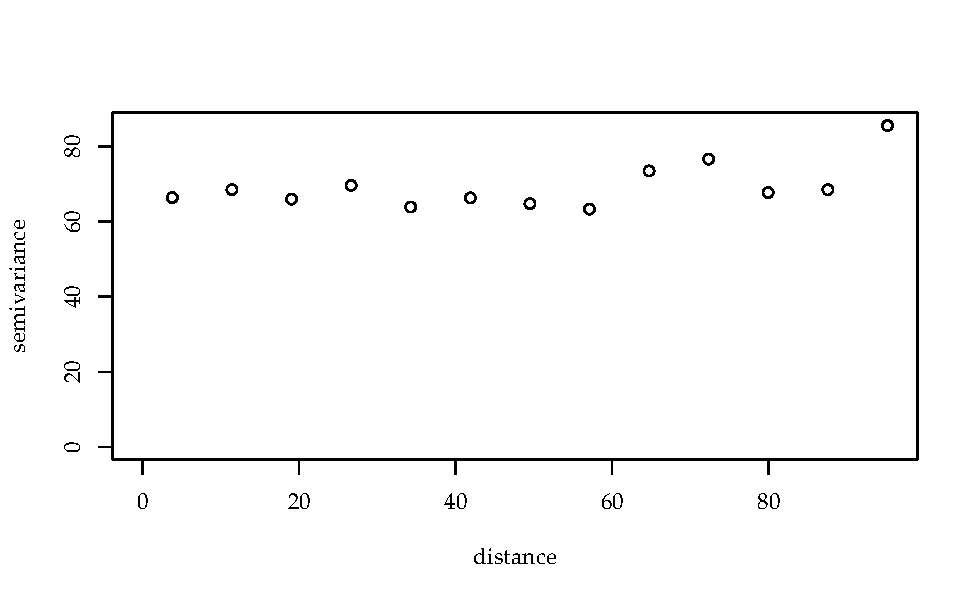
\includegraphics[width=\maxwidth]{figure/prob2c-1} 

}


\begin{kframe}\begin{alltt}
    \hlstd{mean.Zvgram} \hlkwb{<-} \hlkwd{mean}\hlstd{(Zvgram}\hlopt{$}\hlstd{v)}
\end{alltt}
\end{kframe}
\end{knitrout}


The true $\gamma_{z}$(h) =  $\gamma_{e}$(h) = 81. Visually, it appears Materon's estimator in this realization is not on target which is verified by finding the mean of the binned semi-variances, which is  69.2679. On average over many realizations Materon's estimator should be unbiased, but again we only have one realization here. The semi-variances appear to slightly increase towards greater distances


\item {\it Redo the above calculations based on the (still) simple model Zi = 10 + 10i + ei, i.e. there is now a linear trend and the process is no longer stationary.}

\newpage

{\it Compare the empirical semivariogram Zvgram2 to Zvgram. Are the results consistent with part (b) above? Justify your answer.}

The empirical semivariogram Zvgram2 is on a much larger scale than Zvgram and increases with distance. This is consistent with the result in (b), which shows in the presence of a linear spatial trend, the empirical semivariogram is the semivariogram in the presence of no spatial linear trend, plus an extra term that is a function of the difference in means, which in this case is a function of the distance.

\begin{knitrout}\footnotesize
\definecolor{shadecolor}{rgb}{0.969, 0.969, 0.969}\color{fgcolor}\begin{kframe}
\begin{alltt}
\hlkwd{set.seed}\hlstd{(}\hlnum{123}\hlstd{)}
\hlstd{Zdat2}\hlkwb{<-}\hlnum{10} \hlopt{+}\hlnum{10}\hlopt{*}\hlstd{i} \hlopt{+} \hlkwd{rnorm}\hlstd{(}\hlnum{100}\hlstd{,}\hlnum{0}\hlstd{,}\hlnum{9}\hlstd{)}
\hlstd{Zvgram2}\hlkwb{<-}\hlkwd{variog}\hlstd{(}\hlkwc{coords}\hlstd{=xycoord,}\hlkwc{data}\hlstd{=Zdat2)}
\end{alltt}
\begin{verbatim}
variog: computing omnidirectional variogram
\end{verbatim}
\begin{alltt}
\hlkwd{plot}\hlstd{(Zvgram2)}
\end{alltt}
\end{kframe}

{\centering 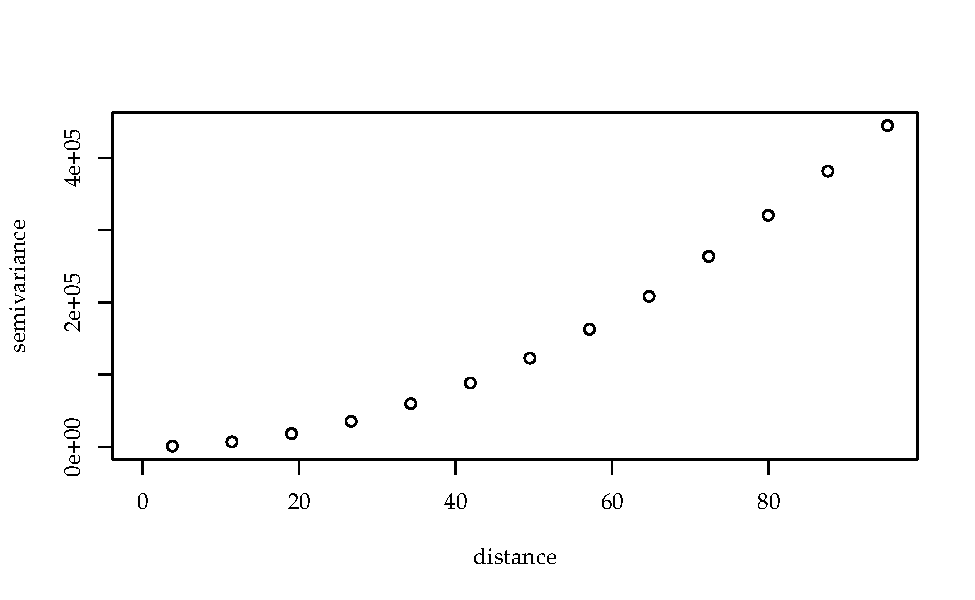
\includegraphics[width=\maxwidth]{figure/prob2d-1} 

}



\end{knitrout}

\item 
{\it Fit a linear model to the data in (d), extract the residuals, and compute the empirical semivariogram for the residuals. Note that what you are doing is removing the trend.}

{\it Compare the 3 empirical semivariograms.}

Once the spatial linear trend is removed, the empirical semi-variogram of the residuals appears to be very similar to the semi-variogram in (c), both in terms of bias and in terms of variation in semi-variances. %even closer to the true semi-variance of 81 and less variable at all distances than the empirical semi-variogram under when fit to the constant mean model. Relative to the semi-variogram without the spaital trend removed, removing the trend and fitting the variogram on the residuals appears to form an unbiased version of the true semi-variance.

Together, relative to the empirical semi-variogram in (c), the semi-variogram of the residuals is very similar. Relative to the empirical semi-variogram in (d), the semi-variogram of the residuals is unbiased with a smaller variance.

\begin{knitrout}\footnotesize
\definecolor{shadecolor}{rgb}{0.969, 0.969, 0.969}\color{fgcolor}\begin{kframe}
\begin{alltt}
\hlstd{e.resid} \hlkwb{<-} \hlkwd{residuals}\hlstd{(}\hlkwd{lm}\hlstd{(Zdat2}\hlopt{~}\hlstd{i))}

\hlstd{evgram} \hlkwb{<-} \hlkwd{variog}\hlstd{(}\hlkwc{coords}\hlstd{=xycoord,}\hlkwc{data}\hlstd{=e.resid)}
\end{alltt}
\begin{verbatim}
variog: computing omnidirectional variogram
\end{verbatim}
\begin{alltt}
\hlkwd{plot}\hlstd{(evgram)}
\end{alltt}
\end{kframe}

{\centering 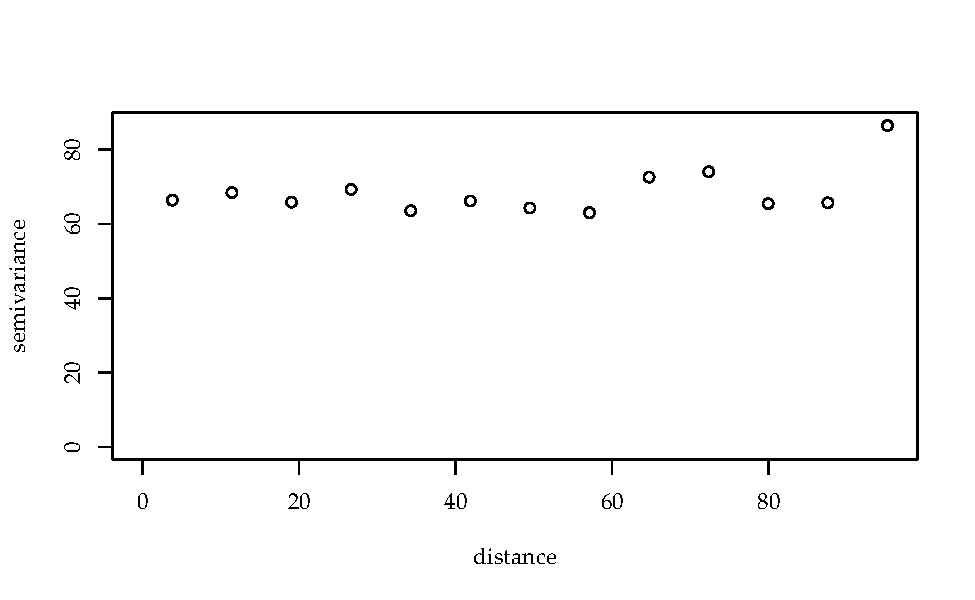
\includegraphics[width=\maxwidth]{figure/prob2e-1} 

}



\end{knitrout}
\end{enumerate}

\item 
{\it Attached is a data set containing the carbon nitrogen values used in the carbon/nitrogen data set. The first 2 columns contain the coordinates, total nitrogen is in the third column, total carbon is in the 4th column and the ratio is in the last column. We will work with the total carbon data. Use geoR for the analysis. It will be easiest if you convert the data into a geodata object as follows.}

\begin{enumerate}
\item {\it Calculate the empirical semivariogram. Give initial eyeball estimates of the nugget effect, sill, and (effective) range.}

The effective range is close to 150, the nugget effect is close to 0.005, and the sill is close to 0.016. The semi-variance does not stabilize for distances greater than a specific point, however, the semi-variance pattern first changes at a distance of 150.


\begin{knitrout}\footnotesize
\definecolor{shadecolor}{rgb}{0.969, 0.969, 0.969}\color{fgcolor}\begin{kframe}
\begin{alltt}
\hlkwd{require}\hlstd{(geoR)}
\hlstd{CN.dat} \hlkwb{<-} \hlkwd{read.table}\hlstd{(}\hlstr{"CN.dat"}\hlstd{,} \hlkwc{header} \hlstd{=} \hlnum{TRUE}\hlstd{)}

\hlcom{# this code created a very different looking semi-variogram}
\hlcom{#data.frame(read.table("CN.dat", header = TRUE))}
\hlcom{#CN.dat[,1] <- as.numeric(CN.dat[,1])}
\hlcom{#CN.dat[,2] <- as.numeric(CN.dat[,2])}
\hlcom{#CN.dat[,2] <- as.numeric(CN.dat[,4])}
\hlcom{#TC.geodata<-as.geodata(CN.dat)#,coords.col=c(1,2),data.col=4)}
\hlcom{#plot(TC.var <- variog(TC.geodata))}

\hlstd{TC.geodata}\hlkwb{<-}\hlkwd{as.geodata}\hlstd{(CN.dat,}\hlkwc{coords.col}\hlstd{=}\hlkwd{c}\hlstd{(}\hlnum{1}\hlstd{,}\hlnum{2}\hlstd{),}\hlkwc{data.col}\hlstd{=}\hlnum{4}\hlstd{)}

\hlkwd{plot}\hlstd{(TC.var} \hlkwb{<-} \hlkwd{variog}\hlstd{(}\hlkwc{coords} \hlstd{= TC.geodata}\hlopt{$}\hlstd{coords,} \hlkwc{data} \hlstd{=} \hlkwd{as.numeric}\hlstd{(TC.geodata}\hlopt{$}\hlstd{data)))}
\end{alltt}
\begin{verbatim}
variog: computing omnidirectional variogram
\end{verbatim}
\end{kframe}

{\centering 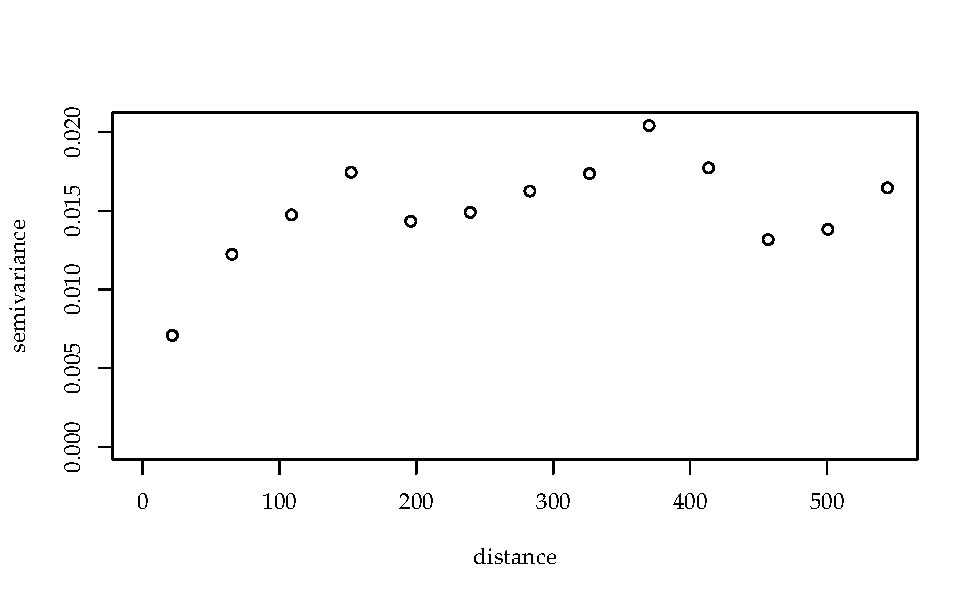
\includegraphics[width=\maxwidth]{figure/prob3a-1} 

}



\end{knitrout}

\item %3b

{\it Fit an exponential semivariogram to the carbon data using OLS, WLS, MLE, and REML methods. Specify a nugget effect in each case, i.e. you do not need to consider models without a nugget. Plot the fitted functions and comment on which one you like best.}

ML and REML both overestimate the sill, OLS and WLS are on target to what I specified as the sill. OLS is simpler, and so is preferred.

\begin{knitrout}\footnotesize
\definecolor{shadecolor}{rgb}{0.969, 0.969, 0.969}\color{fgcolor}\begin{kframe}
\begin{alltt}
\hlcom{# Fitting models estimated nugget}

\hlcom{# partial sill = 0.016-0.005=0.011}
\hlstd{ml.n} \hlkwb{<-} \hlkwd{likfit}\hlstd{(TC.geodata,} \hlkwc{ini} \hlstd{=} \hlkwd{c}\hlstd{(}\hlnum{0.011}\hlstd{,}\hlnum{150}\hlstd{),} \hlkwc{nugget} \hlstd{=} \hlnum{0.005}\hlstd{,} \hlkwc{lik.method} \hlstd{=} \hlstr{"ML"}\hlstd{,} \hlkwc{cov.model} \hlstd{=} \hlstr{"exponential"}\hlstd{,}
               \hlkwc{fix.nug} \hlstd{=} \hlnum{TRUE}\hlstd{)}
\end{alltt}
\begin{verbatim}
kappa not used for the exponential correlation function
---------------------------------------------------------------
likfit: likelihood maximisation using the function optim.
likfit: Use control() to pass additional
         arguments for the maximisation function.
        For further details see documentation for optim.
likfit: It is highly advisable to run this function several
        times with different initial values for the parameters.
likfit: WARNING: This step can be time demanding!
---------------------------------------------------------------
likfit: end of numerical maximisation.
\end{verbatim}
\begin{alltt}
\hlstd{reml.n} \hlkwb{<-} \hlkwd{likfit}\hlstd{(TC.geodata,} \hlkwc{ini} \hlstd{=} \hlkwd{c}\hlstd{(}\hlnum{0.011}\hlstd{,}\hlnum{150}\hlstd{),} \hlkwc{nugget} \hlstd{=} \hlnum{0.005}\hlstd{,} \hlkwc{lik.method} \hlstd{=} \hlstr{"REML"}\hlstd{,}
                  \hlkwc{cov.model} \hlstd{=} \hlstr{"exponential"}\hlstd{,}
               \hlkwc{fix.nug} \hlstd{=} \hlnum{TRUE}\hlstd{)}
\end{alltt}
\begin{verbatim}
kappa not used for the exponential correlation function
---------------------------------------------------------------
likfit: likelihood maximisation using the function optim.
likfit: Use control() to pass additional
         arguments for the maximisation function.
        For further details see documentation for optim.
likfit: It is highly advisable to run this function several
        times with different initial values for the parameters.
likfit: WARNING: This step can be time demanding!
---------------------------------------------------------------
likfit: end of numerical maximisation.
\end{verbatim}
\begin{alltt}
\hlcom{# i chose cressie's weights}
\hlstd{wls.n} \hlkwb{<-} \hlkwd{variofit}\hlstd{(TC.var,} \hlkwc{ini} \hlstd{=} \hlkwd{c}\hlstd{(}\hlnum{0.011}\hlstd{,}\hlnum{150}\hlopt{/}\hlnum{3}\hlstd{),} \hlkwc{weights} \hlstd{=} \hlstr{"cressie"}\hlstd{,}
                  \hlkwc{nugget}\hlstd{=}\hlnum{0.005}\hlstd{,} \hlkwc{cov.model} \hlstd{=} \hlstr{"exponential"}\hlstd{)}
\end{alltt}
\begin{verbatim}
variofit: covariance model used is exponential 
variofit: weights used: cressie 
variofit: minimisation function used: optim 
\end{verbatim}
\begin{alltt}
\hlcom{# equal weights are ols}
\hlstd{ols.n} \hlkwb{<-} \hlkwd{variofit}\hlstd{(TC.var,} \hlkwc{ini} \hlstd{=} \hlkwd{c}\hlstd{(}\hlnum{0.011}\hlstd{,}\hlnum{150}\hlopt{/}\hlnum{3}\hlstd{),} \hlkwc{weights} \hlstd{=} \hlstr{"equal"}\hlstd{,}
                  \hlkwc{nugget}\hlstd{=}\hlnum{0.005}\hlstd{,} \hlkwc{cov.model} \hlstd{=} \hlstr{"exponential"}\hlstd{)}
\end{alltt}
\begin{verbatim}
variofit: covariance model used is exponential 
variofit: weights used: equal 
variofit: minimisation function used: optim 
\end{verbatim}
\begin{alltt}
\hlcom{# Now, plotting fitted models against empirical variogram}
\hlkwd{par}\hlstd{(}\hlkwc{mfrow} \hlstd{=} \hlkwd{c}\hlstd{(}\hlnum{1}\hlstd{,}\hlnum{1}\hlstd{))}
\hlkwd{plot}\hlstd{(TC.var,} \hlkwc{main} \hlstd{=} \hlkwd{expression}\hlstd{(}\hlkwd{paste}\hlstd{(}\hlstr{"Exponential, fixed "}\hlstd{, tau}\hlopt{^}\hlnum{2} \hlopt{==} \hlnum{0.005}\hlstd{)))}
\hlkwd{lines.variomodel}\hlstd{(ml.n,} \hlkwc{max.dist} \hlstd{=} \hlnum{500}\hlstd{)}
\hlkwd{lines}\hlstd{(reml.n,} \hlkwc{lwd} \hlstd{=} \hlnum{2}\hlstd{,} \hlkwc{max.dist} \hlstd{=} \hlnum{500}\hlstd{)}
\hlkwd{lines}\hlstd{(ols.n,} \hlkwc{lty} \hlstd{=} \hlnum{2}\hlstd{,} \hlkwc{max.dist} \hlstd{=} \hlnum{500}\hlstd{)}
\hlkwd{lines}\hlstd{(wls.n,} \hlkwc{lty} \hlstd{=} \hlnum{2}\hlstd{,} \hlkwc{lwd} \hlstd{=} \hlnum{2}\hlstd{,} \hlkwc{max.dist} \hlstd{=} \hlnum{500}\hlstd{)}
\hlkwd{legend}\hlstd{(}\hlnum{300}\hlstd{,} \hlnum{0.008}\hlstd{,} \hlkwc{legend}\hlstd{=}\hlkwd{c}\hlstd{(}\hlstr{"ML"}\hlstd{,}\hlstr{"REML"}\hlstd{,}\hlstr{"OLS"}\hlstd{,}\hlstr{"WLS"}\hlstd{),}\hlkwc{lty}\hlstd{=}\hlkwd{c}\hlstd{(}\hlnum{1}\hlstd{,}\hlnum{1}\hlstd{,}\hlnum{2}\hlstd{,}\hlnum{2}\hlstd{),}\hlkwc{lwd}\hlstd{=}\hlkwd{c}\hlstd{(}\hlnum{1}\hlstd{,}\hlnum{2}\hlstd{,}\hlnum{1}\hlstd{,}\hlnum{2}\hlstd{),} \hlkwc{cex}\hlstd{=}\hlnum{0.7}\hlstd{)}
\end{alltt}
\end{kframe}

{\centering 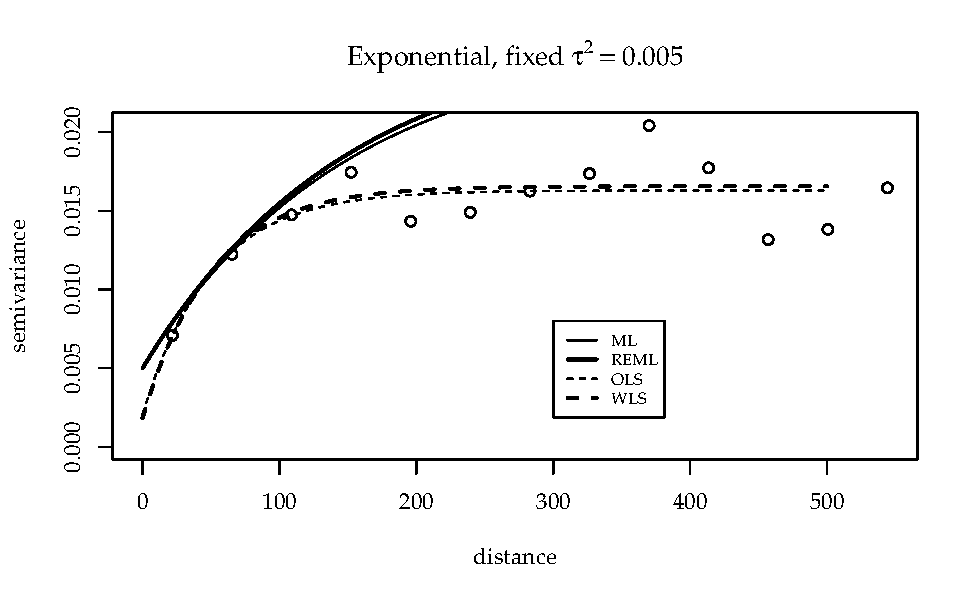
\includegraphics[width=\maxwidth]{figure/prob3b-1} 

}



\end{knitrout}

\item 

With the spherical covariance structure WLS and OLS appear again to do the best at matching the sill I specified and so OLS is againpreferred.


\begin{knitrout}\footnotesize
\definecolor{shadecolor}{rgb}{0.969, 0.969, 0.969}\color{fgcolor}\begin{kframe}
\begin{alltt}
\hlcom{#range itself spherical, range/number exponential}

\hlstd{ml.s} \hlkwb{<-} \hlkwd{likfit}\hlstd{(TC.geodata,} \hlkwc{ini} \hlstd{=} \hlkwd{c}\hlstd{(}\hlnum{0.011}\hlstd{,}\hlnum{150}\hlstd{),} \hlkwc{nugget} \hlstd{=} \hlnum{0.005}\hlstd{,} \hlkwc{lik.method} \hlstd{=} \hlstr{"ML"}\hlstd{,} \hlkwc{cov.model} \hlstd{=} \hlstr{"spherical"}\hlstd{,}
               \hlkwc{fix.nug} \hlstd{=} \hlnum{FALSE}\hlstd{)}
\end{alltt}
\begin{verbatim}
kappa not used for the spherical correlation function
---------------------------------------------------------------
likfit: likelihood maximisation using the function optim.
likfit: Use control() to pass additional
         arguments for the maximisation function.
        For further details see documentation for optim.
likfit: It is highly advisable to run this function several
        times with different initial values for the parameters.
likfit: WARNING: This step can be time demanding!
---------------------------------------------------------------
likfit: end of numerical maximisation.
\end{verbatim}
\begin{alltt}
\hlstd{reml.s} \hlkwb{<-} \hlkwd{likfit}\hlstd{(TC.geodata,} \hlkwc{ini} \hlstd{=} \hlkwd{c}\hlstd{(}\hlnum{0.011}\hlstd{,}\hlnum{150}\hlstd{),} \hlkwc{nugget} \hlstd{=} \hlnum{0.005}\hlstd{,} \hlkwc{lik.method} \hlstd{=} \hlstr{"REML"}\hlstd{,}
                  \hlkwc{cov.model} \hlstd{=} \hlstr{"spherical"}\hlstd{,}
               \hlkwc{fix.nug} \hlstd{=} \hlnum{FALSE}\hlstd{)}
\end{alltt}
\begin{verbatim}
kappa not used for the spherical correlation function
---------------------------------------------------------------
likfit: likelihood maximisation using the function optim.
likfit: Use control() to pass additional
         arguments for the maximisation function.
        For further details see documentation for optim.
likfit: It is highly advisable to run this function several
        times with different initial values for the parameters.
likfit: WARNING: This step can be time demanding!
---------------------------------------------------------------
likfit: end of numerical maximisation.
\end{verbatim}
\begin{alltt}
\hlcom{# i chose cressie's weights}
\hlstd{wls.s} \hlkwb{<-} \hlkwd{variofit}\hlstd{(TC.var,} \hlkwc{ini} \hlstd{=} \hlkwd{c}\hlstd{(}\hlnum{0.011}\hlstd{,}\hlnum{150}\hlstd{),} \hlkwc{weights} \hlstd{=} \hlstr{"cressie"}\hlstd{,}
                  \hlkwc{nugget}\hlstd{=}\hlnum{0.005}\hlstd{,} \hlkwc{cov.model} \hlstd{=} \hlstr{"spherical"}\hlstd{)}
\end{alltt}
\begin{verbatim}
variofit: covariance model used is spherical 
variofit: weights used: cressie 
variofit: minimisation function used: optim 
\end{verbatim}
\begin{alltt}
\hlcom{# equal weights are ols}
\hlstd{ols.s} \hlkwb{<-} \hlkwd{variofit}\hlstd{(TC.var,} \hlkwc{ini} \hlstd{=} \hlkwd{c}\hlstd{(}\hlnum{0.011}\hlstd{,}\hlnum{150}\hlstd{),} \hlkwc{weights} \hlstd{=} \hlstr{"equal"}\hlstd{,}
                  \hlkwc{nugget}\hlstd{=}\hlnum{0.005}\hlstd{,} \hlkwc{cov.model} \hlstd{=} \hlstr{"spherical"}\hlstd{)}
\end{alltt}
\begin{verbatim}
variofit: covariance model used is spherical 
variofit: weights used: equal 
variofit: minimisation function used: optim 
\end{verbatim}
\begin{alltt}
\hlcom{# Now, plotting fitted models against empirical variogram}
\hlkwd{par}\hlstd{(}\hlkwc{mfrow} \hlstd{=} \hlkwd{c}\hlstd{(}\hlnum{1}\hlstd{,}\hlnum{1}\hlstd{))}
\hlkwd{plot}\hlstd{(TC.var,} \hlkwc{main} \hlstd{=} \hlkwd{expression}\hlstd{(}\hlkwd{paste}\hlstd{(}\hlstr{"Spherical, varying "}\hlstd{, tau}\hlopt{^}\hlnum{2}\hlstd{)))}
\hlkwd{lines.variomodel}\hlstd{(ml.s,} \hlkwc{max.dist} \hlstd{=} \hlnum{500}\hlstd{)}
\hlkwd{lines}\hlstd{(reml.s,} \hlkwc{lwd} \hlstd{=} \hlnum{2}\hlstd{,} \hlkwc{max.dist} \hlstd{=} \hlnum{500}\hlstd{)}
\hlkwd{lines}\hlstd{(ols.s,} \hlkwc{lty} \hlstd{=} \hlnum{2}\hlstd{,} \hlkwc{max.dist} \hlstd{=} \hlnum{500}\hlstd{)}
\hlkwd{lines}\hlstd{(wls.s,} \hlkwc{lty} \hlstd{=} \hlnum{2}\hlstd{,} \hlkwc{lwd} \hlstd{=} \hlnum{2}\hlstd{,} \hlkwc{max.dist} \hlstd{=} \hlnum{500}\hlstd{)}
\hlkwd{legend}\hlstd{(}\hlnum{300}\hlstd{,} \hlnum{0.008}\hlstd{,} \hlkwc{legend}\hlstd{=}\hlkwd{c}\hlstd{(}\hlstr{"ML"}\hlstd{,}\hlstr{"REML"}\hlstd{,}\hlstr{"OLS"}\hlstd{,}\hlstr{"WLS"}\hlstd{),}\hlkwc{lty}\hlstd{=}\hlkwd{c}\hlstd{(}\hlnum{1}\hlstd{,}\hlnum{1}\hlstd{,}\hlnum{2}\hlstd{,}\hlnum{2}\hlstd{),}\hlkwc{lwd}\hlstd{=}\hlkwd{c}\hlstd{(}\hlnum{1}\hlstd{,}\hlnum{2}\hlstd{,}\hlnum{1}\hlstd{,}\hlnum{2}\hlstd{),} \hlkwc{cex}\hlstd{=}\hlnum{0.7}\hlstd{)}
\end{alltt}
\end{kframe}

{\centering 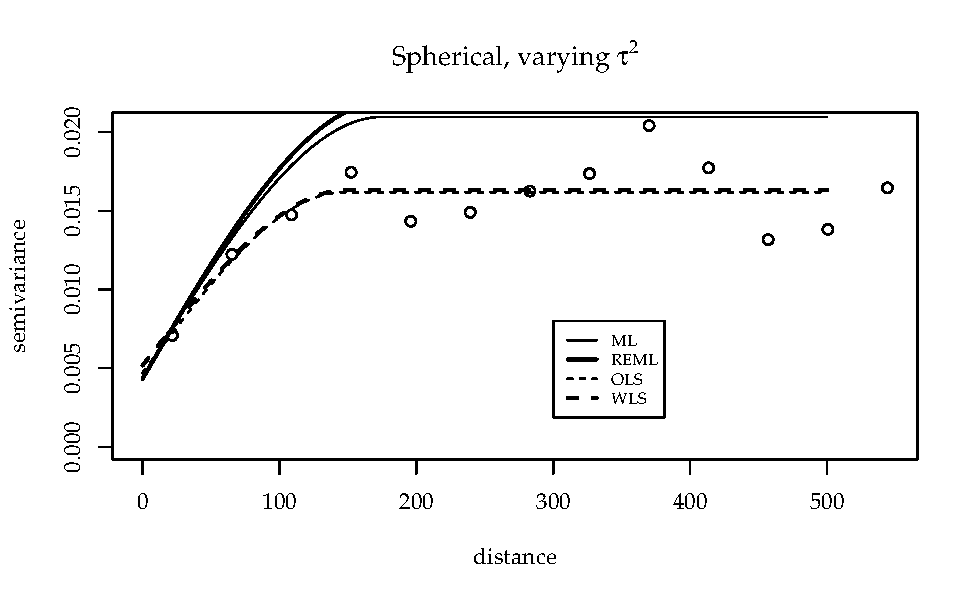
\includegraphics[width=\maxwidth]{figure/prob3c-1} 

}



\end{knitrout}

\newpage

\item

{\it Summarize your results in table format. Compare the results and discuss.}

The practical range and partial sill are overestimated for the ML and REML methods with the spherical covariance structure. OLS and WLS approximate the practical range and partial sill very closely with the spherical covariance model. All methods do well in estimating the nugget effect based on what I specified.

\begin{kframe}
\begin{alltt}
\hlstd{var.outn} \hlkwb{<-} \hlkwd{data.frame}\hlstd{(}\hlkwd{cbind}\hlstd{(}\hlkwd{c}\hlstd{(ml.n}\hlopt{$}\hlstd{parameters.summary[}\hlkwd{c}\hlstd{(}\hlnum{2}\hlstd{,}\hlnum{3}\hlstd{,}\hlnum{4}\hlstd{),}\hlnum{2}\hlstd{]),}
                             \hlkwd{c}\hlstd{(reml.n}\hlopt{$}\hlstd{parameters.summary[}\hlkwd{c}\hlstd{(}\hlnum{2}\hlstd{,}\hlnum{3}\hlstd{,}\hlnum{4}\hlstd{),}\hlnum{2}\hlstd{]),}
                             \hlkwd{c}\hlstd{(}\hlkwd{t}\hlstd{(}\hlkwd{summary}\hlstd{(wls.s)}\hlopt{$}\hlstd{estimated.pars)),}
                             \hlkwd{c}\hlstd{(}\hlkwd{t}\hlstd{(}\hlkwd{summary}\hlstd{(wls.s)}\hlopt{$}\hlstd{estimated.pars))))}
\hlkwd{colnames}\hlstd{(var.outn)} \hlkwb{<-} \hlkwd{c}\hlstd{(}\hlstr{"ML Exp"}\hlstd{,} \hlstr{"REML Exp"}\hlstd{,} \hlstr{"OLS Exp"}\hlstd{,} \hlstr{"WLS Exp"}\hlstd{)}
\hlkwd{rownames}\hlstd{(var.outn)} \hlkwb{<-} \hlkwd{c}\hlstd{(}\hlstr{"nugget"}\hlstd{,} \hlstr{"part. sill"}\hlstd{,} \hlstr{"pract. range"}\hlstd{)}


\hlstd{var.out} \hlkwb{<-} \hlkwd{data.frame}\hlstd{(}\hlkwd{cbind}\hlstd{(}\hlkwd{c}\hlstd{(ml.s}\hlopt{$}\hlstd{parameters.summary[}\hlkwd{c}\hlstd{(}\hlnum{2}\hlstd{,}\hlnum{3}\hlstd{,}\hlnum{4}\hlstd{),}\hlnum{2}\hlstd{]),}
                            \hlkwd{c}\hlstd{(reml.s}\hlopt{$}\hlstd{parameters.summary[}\hlkwd{c}\hlstd{(}\hlnum{2}\hlstd{,}\hlnum{3}\hlstd{,}\hlnum{4}\hlstd{),}\hlnum{2}\hlstd{]),}
                            \hlkwd{c}\hlstd{(}\hlkwd{t}\hlstd{(}\hlkwd{summary}\hlstd{(ols.s)}\hlopt{$}\hlstd{estimated.pars)),}
                            \hlkwd{c}\hlstd{(}\hlkwd{t}\hlstd{(}\hlkwd{summary}\hlstd{(ols.s)}\hlopt{$}\hlstd{estimated.pars))))}
\hlkwd{colnames}\hlstd{(var.out)} \hlkwb{<-} \hlkwd{c}\hlstd{(}\hlstr{"ML Sphere"}\hlstd{,} \hlstr{"REML Sphere"}\hlstd{,} \hlstr{"OLS Sphere"}\hlstd{,} \hlstr{"WLS Sphere"}\hlstd{)}
\hlkwd{rownames}\hlstd{(var.out)} \hlkwb{<-} \hlkwd{c}\hlstd{(}\hlstr{"nugget"}\hlstd{,}\hlstr{"part. sill"}\hlstd{,} \hlstr{"pract. range"}\hlstd{)}

\hlkwd{print}\hlstd{(}\hlkwd{xtable}\hlstd{(var.outn,} \hlkwc{align} \hlstd{=} \hlstr{"||l|l|l|l|l||"}\hlstd{,} \hlkwc{digits} \hlstd{=} \hlkwd{c}\hlstd{(}\hlnum{6}\hlstd{,}\hlnum{6}\hlstd{,}\hlnum{6}\hlstd{,}\hlnum{6}\hlstd{,}\hlnum{6}\hlstd{)))}
\end{alltt}
\end{kframe}% latex table generated in R 3.3.2 by xtable 1.8-2 package
% Fri Feb 17 11:18:37 2017
\begin{table}[ht]
\centering
\begin{tabular}{||l|l|l|l|l||}
  \hline
 & ML Exp & REML Exp & OLS Exp & WLS Exp \\ 
  \hline
nugget & 0.005000 & 0.005000 & 0.005171 & 0.005171 \\ 
  part. sill & 0.021000 & 0.021500 & 0.011160 & 0.011160 \\ 
  pract. range & 150.000000 & 150.000000 & 150.000000 & 150.000000 \\ 
   \hline
\end{tabular}
\end{table}
\begin{kframe}\begin{alltt}
\hlkwd{print}\hlstd{(}\hlkwd{xtable}\hlstd{(var.out,} \hlkwc{align} \hlstd{=} \hlstr{"||l|l|l|l|l||"}\hlstd{,} \hlkwc{digits} \hlstd{=} \hlkwd{c}\hlstd{(}\hlnum{6}\hlstd{,}\hlnum{6}\hlstd{,}\hlnum{6}\hlstd{,}\hlnum{6}\hlstd{,}\hlnum{6}\hlstd{)))}
\end{alltt}
\end{kframe}% latex table generated in R 3.3.2 by xtable 1.8-2 package
% Fri Feb 17 11:18:37 2017
\begin{table}[ht]
\centering
\begin{tabular}{||l|l|l|l|l||}
  \hline
 & ML Sphere & REML Sphere & OLS Sphere & WLS Sphere \\ 
  \hline
nugget & 0.004500 & 0.004300 & 0.004705 & 0.004705 \\ 
  part. sill & 0.016500 & 0.017600 & 0.011475 & 0.011475 \\ 
  pract. range & 174.823700 & 176.065700 & 147.305888 & 147.305888 \\ 
   \hline
\end{tabular}
\end{table}


\end{enumerate}
\end{enumerate}

\end{document}

